\documentclass[12pt]{article}

% set margins
\usepackage[letterpaper, margin=1in]{geometry}

% set spacing
\usepackage{setspace}

% hyperlinks
\usepackage{hyperref}
\hypersetup{colorlinks, citecolor={black},	
linkcolor={blue}, urlcolor={blue}}

% endnotes
\usepackage{endnotes}
\let\footnote=\endnote

% set image attributes
\usepackage{graphicx}
\graphicspath{ {images/} }
\usepackage{float}
\usepackage{placeins}

% for sample paper ONLY
\usepackage{lipsum}

% ============================================================

% define the title
\title{Sample Paper Title}
\author{Christopher G. Prener, Ph.D.}
\date{}

% ============================================================

\begin{document}

% ============================================================

\maketitle

\vspace{10mm}
\par \noindent \textit{Corresponding Author:}
\par \noindent Christopher G. Prener, Ph.D.
\par \noindent Assistant Professor of Sociology
\par \noindent Saint Louis University
\par \noindent \href{chris.prener@slu.edu}{chris.prener@slu.edu}

\vspace{5mm}
\par \noindent \textit{Mailing Address:}
\par \noindent 1900 Morrissey Hall
\par \noindent 3700 Lindell Blvd
\par \noindent St. Louis, MO 63108

% ======================================================

\begin{doublespace}

% ======================================================

\newpage
\section*{Abstract}
\lipsum[1]

\newpage
\lipsum[2-3]

% ======================================================

\vspace{5mm}
\section*{Background}
\lipsum[4]

\vspace{3mm}
\subsection*{Subsection 1}
\lipsum[5-6]

\vspace{3mm}
\subsection*{Subsection 2}
\lipsum[7-8]

\vspace{3mm}
\subsection*{Hypotheses}
\lipsum[9]

\begin{itemize}
\item H\textsubscript{1} - Suspendisse vitae elit.
\item H\textsubscript{2} - Aliquam arcu neque, ornare in, ullamcorper quis, commodo eu, libero.\footnote{Maecenas sapien libero, molestie et, lobortis in, sodales eget, dui.}
\end{itemize}

\lipsum[11]

\vspace{5mm}
\section*{Data \& Methods}
\subsection*{Data}
\lipsum[12-13]

\begin{center}
$<<<<<<<<<<$ Table \ref{tbl:descriptiveStats} (see p. \pageref{tbl:descriptiveStats}) about here $>>>>>>>>>>$
\end{center}

\vspace{3mm}
\subsection*{Methods}
\lipsum[14-16]

\vspace{5mm}
\section*{Results}
\lipsum[17-19]

\begin{center}
$<<<<<<<<<<$ Figure \ref{fig:exampleFigure} (see p. \pageref{fig:exampleFigure}) about here $>>>>>>>>>>$
\end{center}

\lipsum[20]

\vspace{5mm}
\section*{Discussion}
\lipsum[21-22]

\vspace{3mm}
\subsection*{Limitations}
\lipsum[23]

\vspace{5mm}
\section*{Conclusion}
\lipsum[24]

% ======================================================

\end{doublespace}

% ======================================================

\newpage

\theendnotes

% ======================================================

\newpage
\section*{Tables}
\begin{table}[!htbp] \centering 
  \caption{Descriptive Statistics} 
  \label{tbl:descriptiveStats} 
\begin{tabular}{@{\extracolsep{5pt}}lccccc} 
\\[-1.8ex]\hline 
\hline \\[-1.8ex] 
Statistic & \multicolumn{1}{c}{N} & \multicolumn{1}{c}{Mean} & \multicolumn{1}{c}{St. Dev.} & \multicolumn{1}{c}{Min} & \multicolumn{1}{c}{Max} \\ 
\hline \\[-1.8ex] 
Displacement & 234 & 3.472 & 1.292 & 1.600 & 7.000 \\ 
Year & 234 & 2,003.500 & 4.510 & 1,999 & 2,008 \\ 
Cylinders & 234 & 5.889 & 1.612 & 4 & 8 \\ 
Fuel Efficiency, City & 234 & 16.859 & 4.256 & 9 & 35 \\ 
Fuel Efficiency, Highway & 234 & 23.440 & 5.955 & 12 & 44 \\ 
\hline \\[-1.8ex] 
\end{tabular} 
\end{table} 

% ======================================================

\newpage
\section*{Figures}
\begin{figure}[H]
  \caption{Example figure - a histogram of \texttt{hwy}}
  \label{fig:exampleFigure}
  \centering
  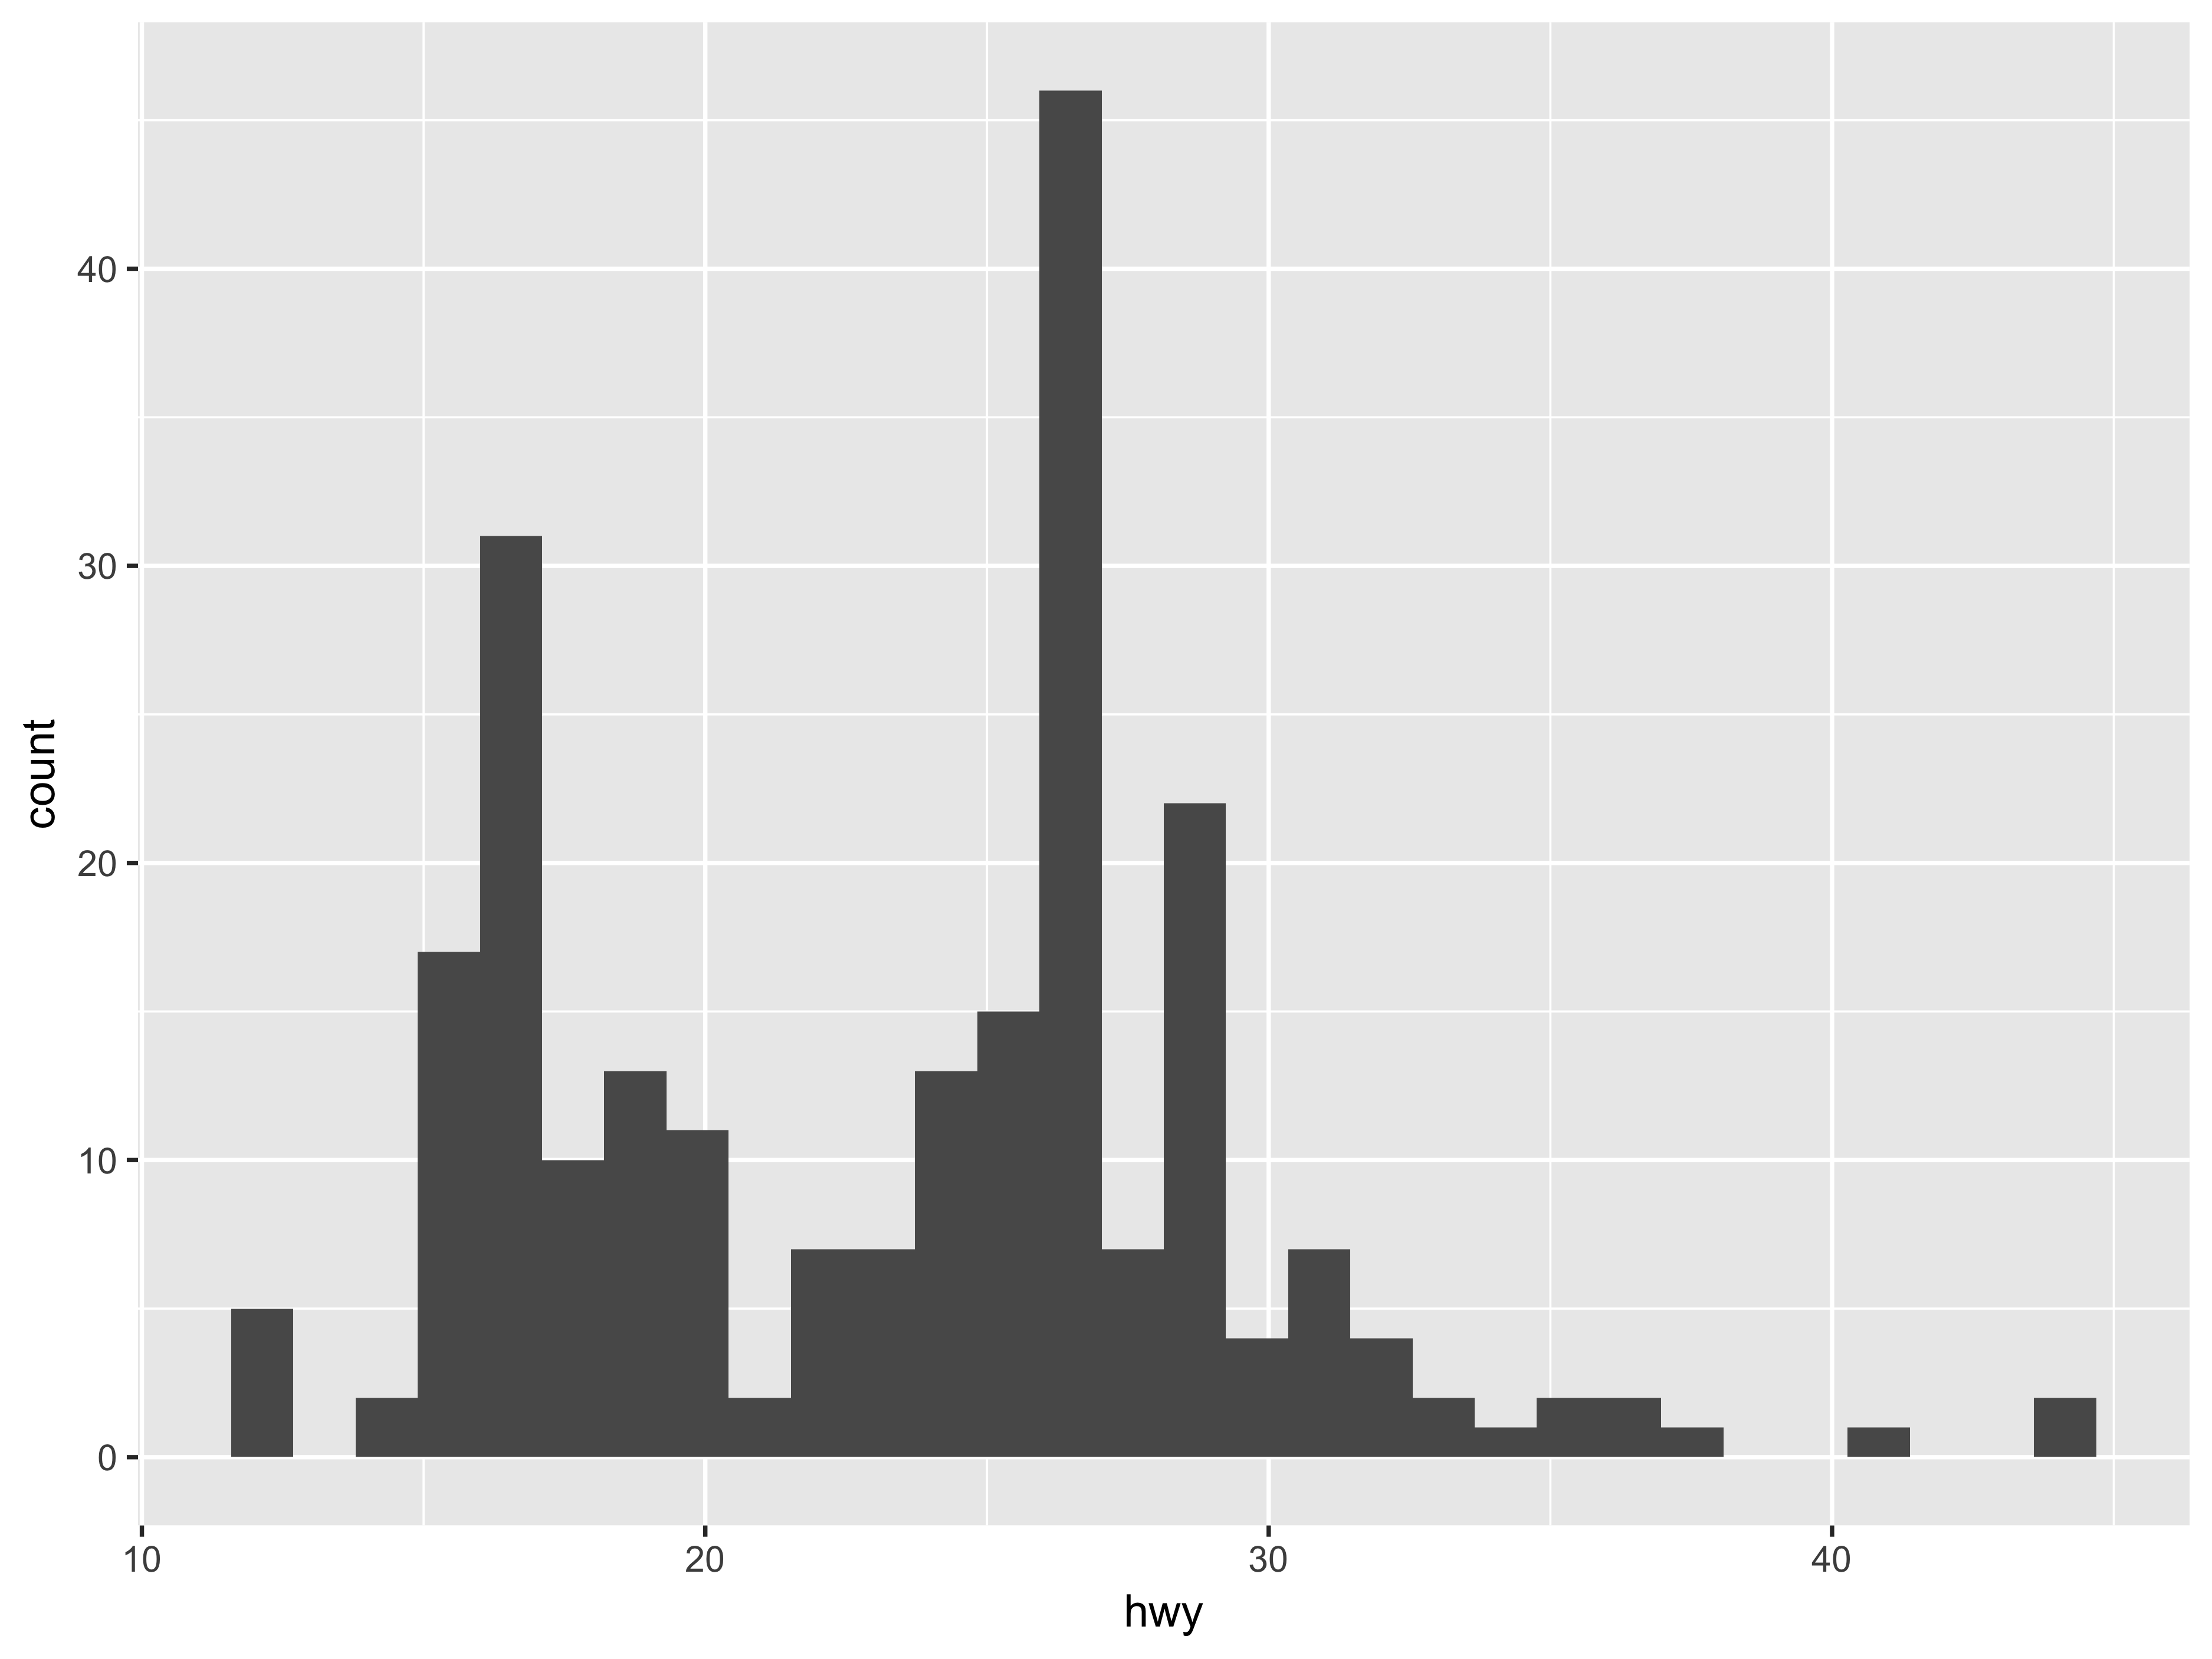
\includegraphics[scale=0.125]{exampleFigure.png}
\end{figure}

\FloatBarrier

% ======================================================

\end{document}